\documentclass{beamer}

\usetheme{Madrid}
\setbeamertemplate{navigation symbols}{}
\setbeamertemplate{caption}[numbered]


\usepackage{graphicx}
\usepackage{amsmath}
\usepackage{xeCJK}
\usepackage{booktabs}
\usepackage{multirow}
\usepackage{tikz}
\usepackage{makecell}


\title[Necessary Conditions of Political Unification]{External Threats, Linguistic Homogeneity, and Political Unification}
\author{Chen Zeng}
\institute[]{Department of Political Science \\ Renmin University of China}

\begin{document}
	\maketitle
	\begin{frame}{Introduction}
		\begin{columns}
			\begin{column}{.4\textwidth}
				
\includegraphics[width=\textwidth]{santa_croce.jpg}
				\scriptsize
				\centering
				Basilica di Santa Croce
			\end{column}
			\begin{column}{.6\textwidth}
				Niccolò Machiavelli, a Florentine in the 16th century, argued for the unification of Italy, which didn't happen until the \textit{Risorgimento} in 19th century, citing the following reasons:
				\begin{itemize}
					\item Florentine lifestyle
					\item The Italian language, esp. Tuscan dialect
					\item Women, god, and heroes
					\item External interference
				\end{itemize}
			\end{column}
		\end{columns}
	\end{frame}

	\begin{frame}{Introduction}
		\begin{itemize}
			\item The English word ``nation'' comes from Latin \textit{nātiōnem}, accusative of \textit{nātiō}, equivalent to \textit{nāscor} (``to be born'') +‎ -\textit{tiō} (``verbal abstract noun suffix'').
			\item In Chinese, the word for country/nation/state is ``国''; it is a geopolitical concept, focusing on the territory and political power.
			\begin{itemize}
				\item 《说文》记载:``古或國同用。''
				\item 根据《字源》中的考察,``或''从口从戈,``口''代表疆土,而``戈''则是兵器;后来``或''被假借为或许、疑惑之意,才又造出``國''字来。
				\item 《周礼注》中又说:``大曰邦,小曰國;邦之所居亦曰國。''
			\end{itemize}
			\item Today we look at two key elements in the political unification of states---external security threats and linguistic homogeneity.
		\end{itemize}
	\end{frame}


	\begin{frame}{Contents}
		\tableofcontents
	\end{frame}
	\section{Conceptualization and Operationalization}
	\subsection{Political Unification}
	\begin{frame}{Political Unification}
		\begin{block}{Definition}
			\begin{description}
				\item[Political unification] occurs when two or more sovereign states merge into one.
			\end{description}
		\end{block}
		\begin{itemize}
			\item Political unification has been one of the most debated areas in the study of political science.
			\item Notable instances included the US (American Revolutionary War), Germany (\textit{Sonderweg}), and Italy (\textit{Risorgimento}).
			\item Does the unification happen incrementally, or is there a clear moment for such unification?
			\item Recent development of the EU, free trade areas, and customs unions has led political scientists to examine if there are limits to such political and economic integration. To which point do they stop being just ``integration'' and become unification?
		\end{itemize}
	\end{frame}
	\begin{frame}{Political Unification}
		\begin{itemize}
			\item An \textit{operational} definition of political unification used in this article is that two sovereign states voluntarily merge into a federation or unitary state. Conquests/accessions are excluded.
			\begin{description}
				\item[Unit of analysis] Political unification (of a state dyad)
				\item[Unit of observation] Inter-state actions (dichotomous variable: unification, linguistic homogeneity); and individual states (continuous variable: threat levels)
			\end{description}
		\end{itemize}

		\begin{itemize}
			\item This research leverages datasets from the Correlates of War project. Qualifying states have to meet at least one of the following criteria.
			\begin{description}
				\item[Criterion 1] Before 1920, a population of at least 500,000 and establishment of diplomatic missions at or above the rank of \textit{chargé d'affaires} by Britain and France.
				\item[Criterion 2] After 1920, membership in the League of Nations or United Nations \textit{or} a population of at least 500,000 and establishment of diplomatic missions from any two major powers.
			\end{description}
		\end{itemize}
	\end{frame}




	\subsection{External Security Threats}
	\begin{frame}{External Security Threats}
		\begin{itemize}
			\item Riker (1975) argues that states unify for security reasons; they desire protection from external threats.
			\item The underlying logic is that sovereignty is a valuable possession and only security-related factors will induce states to give it up voluntarily.
			\item With its roots in the realist tradition, this position has been supported and extended in a series of studies that address the problem theoretically, formally, and through case studies (Deudney 1995; Hechter 2000; Parent 2009; Rector 2009; Stepan 2001).
			\item the notion that security issues are a necessary condition for political unification has become somewhat of a conventional wisdom.
		\end{itemize}
	\end{frame}
	\subsection{Linguistic Homogeneity}
	\begin{frame}{Linguistic Homogeneity}
		\begin{itemize}
			\item A common language can be posited as a necessary condition for political unification. The logic is that states will have an easier time understanding one another, and can imagine themselves as part of a larger group or nation.
			\item Language can be thought of as proxy for other culturally relevant factors such as nation or ethnicity. Although the distribution of languages does not correspond perfectly with nation or ethnicity, but there is a strong relationship, and language is more identifiable marker.
			\item To certain extent, the hypotheses of security threats and linguistic homogeneity having impact on political unification reflect the realist-constructionist divide.
		\end{itemize}
	\end{frame}


	\begin{frame}{Research Hypotheses}
		\begin{description}
			\item[Hypothesis 1] External threats are \textit{necessary} for political unification.
			\item[Hypothesis 2] Linguistic homogeneity is \textit{necessary} for political unification.
		\end{description}
		\begin{itemize}
			\item The article takes on the form of a \textit{falsification} probe and focuses on only \textit{necessary} conditions for political unification.
			\item That is to say that security threats or linguistic homogeneity may not be \textit{sufficient} for political unification, but the lack of either condition cannot result in the expected outcome.
			\item This method is prone to many methodological and substantive vulnerabilities. We will cover them in the final section, but now, let's take a look into why the author sets those two key explanatory variables.
		\end{itemize}
	\end{frame}
	\section{Analysis}
	\subsection{Cases of Unification}
	\begin{frame}{Cases of Unification}
		\begin{table}
			\centering
			\footnotesize
			\caption{Cases of Unification after 1816}
			\begin{tabular}{lr}
				\toprule
				Event & Year \\
				\midrule
				Piedmont -- Parma & 1860 \\
				Piedmont -- Tuscany & 1860 \\
				Piedmont -- Modena & 1860 \\
				Prussia -- Mecklenburg Schwerin & 1867 \\
				Prussia -- Hesse Grand Ducal & 1867 \\
				Prussia -- Baden & 1871 \\
				Prussia -- Bavaria & 1871 \\
				Prussia -- Wuerttemburg & 1871 \\
				France -- Tunisia & 1881 \\
				Japan -- Korea & 1905 \\
				USA -- Cuba & 1906 \\
				Egypt -- Syria & 1958 \\
				Tanganyika -- Zanzibar & 1964 \\
				West Germany -- East Germany & 1990 \\
				Yemen Arab Republic -- Yemen People's Republic & 1990 \\
				\bottomrule
			\end{tabular}
		\end{table}
	\end{frame}
	\subsection{Testing Security Hypothesis}
	\begin{frame}{Within-state Comparisons}
		\begin{table}
			\centering
			\caption{Within-state Comparisons}
			\tiny
			\begin{tabular}{lcccc}
				\toprule
				State & \makecell{Threat Level \\ (Overall)} & Unification Year & \makecell{Threat Level \\ (Pre-unification)} & Threat Differential \\
				\midrule
				Egypt & 2.5 & 1958 & 11.3 & 8.8$^{***}$ \\
				Syria & 12.2 & 1958 & 20.3 & 8.1$^{**}$ \\
				Prussia & 1.4 & 1867, 1871 & 4.5 & 3.1$^{**}$ \\
				Piedmont & 1.0 & 1860 & 4.0 & 3$^{**}$ \\
				Hesse Grand Ducal & 0.2 & 1867 & 2.0 & 1.8$^{***}$ \\
				Mecklenburg-Schwerin & 0.2 & 1867 & 1.3 & 1.1$^{**}$ \\
				Baden & 0.2 & 1871 & 1.3 & 1.1$^{**}$ \\
				Bavaria & 0.3 & 1871 & 1.3 & 1$^{*}$ \\
				Wuerttemburg & 0.4 & 1871 & 1.3 & 0.9 \\
				
				Parma & 0.0 & 1860 & 0.0 & 0.0 \\
				Zanzibar & 0.0 & 1864 & 0.0 & 0.0 \\
				Tanganyika & 0.0 & 1864 & 0.0 & 0.0 \\
				Tuscany & 0.1 & 1860 & 0.0 & -0.1 \\
				Modena & 0.3 & 1860 & 0.0 & -0.3 \\
				West Germany & 1.0 & 1990 & 0.5 & -0.5 \\
				Yemen Arab Republic & 1.7 & 1990 & 1.0 & -0.73 \\
				East Germany & 0.9 & 1990 & 0.0 & -0.9 \\
				Yemen People's Republic & 2.2 & 1990 & 0.0 & -2.2$^{*}$ \\
				\bottomrule
				\\[-1.8ex] 
				\textit{Note:} & \multicolumn{4}{r}{$^{*}$p$<$0.1; $^{**}$p$<$0.05; $^{***}$p$<$0.01} \\
			\end{tabular}
		\end{table}
	\end{frame}
	\subsection{Testing Linguistic Homogeneity Hypothesis}

	\begin{frame}
		\begin{table}
			\centering
			\footnotesize
			\caption{Linguistic Homogeneity of Unifying States}
			\begin{tabular}{lcc}
				\toprule
				Event & Year & Linguistic Homogeneity\\
				\midrule
				Piedmont -- Parma & 1860 & Yes$^*$ \\
				Piedmont -- Tuscany & 1860 & Yes$^*$ \\
				Piedmont -- Modena & 1860 & Yes$^*$ \\
				Prussia -- Mecklenburg Schwerin & 1867 & Yes \\
				Prussia -- Hesse Grand Ducal & 1867 & Yes \\
				Prussia -- Baden & 1871 & Yes$^*$ \\
				Prussia -- Bavaria & 1871 & Yes$^*$ \\
				Prussia -- Wuerttemburg & 1871 & Yes$^*$ \\
				France -- Tunisia & 1881 & No \\
				Japan -- Korea & 1905 & No \\
				USA -- Cuba & 1906 & No \\
				Egypt -- Syria & 1958 & Yes \\
				Tanganyika -- Zanzibar & 1964 & Yes \\
				West Germany -- East Germany & 1990 & Yes \\
				Yemen Arab Republic -- Yemen People's Republic & 1990 & Yes \\
				\bottomrule
				\\[-1.8ex] 
				\textit{Note:} & \multicolumn{2}{r}{$^*$Borderline case} \\
			\end{tabular}
		\end{table}
	\end{frame}

	\section{Reflections}
	\begin{frame}{Reflections}
		In the following subsections, we let \textit{U} denote political unification, \textit{S} external security threats, and \textit{L} linguistic homogeneity.
		\begin{itemize}
			\item From previous analysis, the author detected 12 cases of political unification from the MID dataset, where linguistic homogeneity is present in all cases. Incorporating the Switzerland case as an outlier, we have 13 cases in total. Mathematically, we have
			\begin{equation}
				P(L|U)=\frac{12}{13} \approx 0.92
			\end{equation}
			\item According to Bayes theorem, we have 
			\begin{equation}
				P(U|L)=\frac{P(U)P(L|U)}{P(L)}
			\end{equation}
		\end{itemize}
	\end{frame}
	\begin{frame}{Reflections}
		\begin{itemize}
			\item Since $P(U)$ and $P(L)$ have the same denominator, we can simplify the equation as
			\begin{equation}
				P(U|L)=\frac{N(U)P(L|U)}{N(L)}
			\end{equation}
			whereas $N(U)=12$, as per previous discussion.
			\item Only considering all 6 UN official languages, we have
			\begin{equation}
%				EN: 19, ES: 20, FR: 29, RU: 5, AR: 22, ZH: 2
				\begin{aligned}
					N(L)< & N(EN)^2 + N(ES)^2 + N(FR)^2 + N(ZH)^2 + \\
					& N(RU)^2 + N(AR)^2 = 2115
				\end{aligned}
			\end{equation}
			\item Furthermore, we estimate the probability of political unification given the presence of linguistic homogeneity.
			\begin{equation}
				P(U|L)=\frac{N(U)P(L|U)}{N(L)}<\frac{12\times 0.92}{2115}\approx 0.52\%
			\end{equation}
		\end{itemize}
	\end{frame}

	\begin{frame}{Causal Inference}
		\begin{itemize}
			\item Before we investigate why there is a significant gap between those two probabilities, we first consider how we should draw causal inference of political unification, taking two variables---external threats, and linguistic homogeneity---into consideration.
		\end{itemize}
		\begin{table}[h]
			\centering
			\caption{Potential Outcomes of Political Unification}
			\begin{tabular}{ccc}
				\toprule
				 & \multicolumn{2}{c}{External Threats} \\
				\cmidrule{2-3}
				Linguistic Homogeneity & No & Yes \\
				\midrule
				No & $Y(0,0)=?$  & $Y(1,0)=?$ \\
				Yes & $Y(0,1)=?$ & $Y(1,1)=?$ \\
				\bottomrule
			\end{tabular}
		\end{table}
		\begin{itemize}
			\item We first present a counterfactual analysis, and then try to relax the requirements for our evidence. As we do it, we are making stronger assumptions to draw causal inference.
		\end{itemize}
	\end{frame}
	
	\begin{frame}{Causal Inference}
		\begin{block}{The Fundamental Problem of Causal Inference}
			This problem arises because we can't observe counterfactual outcomes; instead, we can only observe one of the potential outcomes.
		\end{block}
		\begin{itemize}
			\item Research designs for causal inference, each has its own assumptions (from weak to strong)
			\begin{itemize}
				\item Randomized Control Experiment (RCT, true randomization, assumes unit homogeneity) --- usually not possible for macro-level researches in social sciences
				\item Natural experiment (as-if randomization) --- not applicable to this research question
				\item Observational study
				\begin{itemize}
					\item Problems: spurious relationships, omitted-variable bias, endogeneity, strong assumptions
					\item Possible solutions: regression discontinuity design (RDD), difference in differences (DiD), instrumental variable (IV)...
				\end{itemize}
			\end{itemize}
		\end{itemize}
	\end{frame}
	
	\subsection{Selection Bias}
	\begin{frame}{Selection Bias}
		\begin{itemize}
			\item The problem of \textit{external validity}---does the conclusion we draw from the sample also apply to the population?
			\item The sample used in this article is \textit{not} representative---it only uses evidence available after 1816, ignoring key cases such as the American Revolutionary War. This is not a random sample.
			\item Omitted-variable bias is present. Other factors that may influence political unification are not controlled. Interaction cannot be taken into consideration in current research framework.
			\item Possible presence of confounding variables.
		\end{itemize}
	\end{frame}
	\subsection{Confounding Factors -- Geographical Proximity}
	
	
	\begin{frame}{Confounding factors -- geographical proximity}
		\begin{figure}
		\centering
			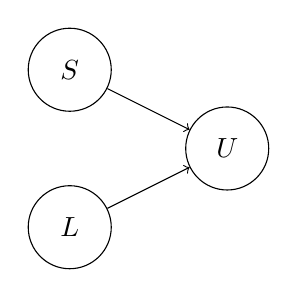
\begin{tikzpicture}[node distance = 3cm, auto]
				\node[circle,
				minimum width = 30pt,
				minimum height = 30pt, draw=black] (1) at(0,1){$S$};
				\node[circle,
				minimum width = 30pt,
				minimum height = 30pt, draw=black] (2) at(0,-1){$L$};
				\node[circle,
				minimum width = 30pt,
				minimum height = 30pt, draw=black] (3) at(2,0){$U$};
				\draw[->] (1) -- (3);
				\draw[->] (2) -- (3);
			\end{tikzpicture}
			\caption{Causal Diagram of Griffith's Paper}
		\end{figure}
	\end{frame}

	\begin{frame}{Confounding factors -- geographical proximity}
		\begin{figure}
			\centering
			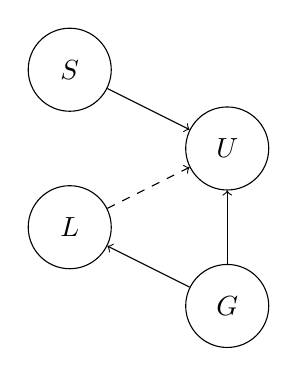
\begin{tikzpicture}[node distance = 3cm, auto]
				\node[circle,
				minimum width = 30pt,
				minimum height = 30pt, draw=black] (1) at(0,1){$S$};
				\node[circle,
				minimum width = 30pt,
				minimum height = 30pt, draw=black] (2) at(0,-1){$L$};
				\node[circle,
				minimum width = 30pt,
				minimum height = 30pt, draw=black] (3) at(2,0){$U$};
				\node[circle,
				minimum width = 30pt,
				minimum height = 30pt, draw=black] (4) at(2,-2){$G$};
				\draw[->] (1) -- (3);
				\draw[->,dashed] (2) -- (3);
				\draw[->] (4) -- (2);
				\draw[->] (4) -- (3);
			\end{tikzpicture}
			\caption{Causal Diagram with Spatial Proximity as A Confounder}
		\end{figure}
		\begin{equation*}
			\begin{aligned}
				\text{wherein, } & Cov(L,G)\neq 0 \\
				& Cov(U,G)\neq 0
			\end{aligned}
		\end{equation*}
	\end{frame}


	\subsection{Alternative Research Design -- QCA \& Logistic Regression}
	\begin{frame}{Alternative research design -- csQCA}
		\begin{table}
			\centering
			\caption{Aggregated Political Unification Cases}
			\begin{tabular}{ccccc}
				\toprule
				& \multicolumn{2}{c}{Explanatory} & Outcome & \\
				\cmidrule(lr){2-3} \cmidrule(lr){4-4} 
				 & S & L & U & Cases \\
				\midrule
				1 & No & No & ? & ? \\
				2 & No & Yes & ? & ? \\
				3 & Yes & No & ? & ? \\
				4 & Yes & Yes & ? & ? \\
				\bottomrule
			\end{tabular}
		\end{table}
	\end{frame}

	\begin{frame}{Alternative research design -- csQCA}
		\begin{table}
			\centering
			\caption{Aggregated Political Unification Cases (Hypothetical Scenario)}
			\begin{tabular}{ccccc}
				\toprule
				& \multicolumn{2}{c}{Explanatory} & Outcome & \\
				\cmidrule(lr){2-3} \cmidrule(lr){4-4} 
				& S & L & U & Cases \\
				\midrule
				1 & No & No & No & 800 \\
				2 & No & Yes & Yes & 50 \\
				3 & Yes & No & Yes & 100 \\
				4 & Yes & Yes & Yes & 12 \\
				\bottomrule
			\end{tabular}
		\end{table}
		\begin{equation}
			\begin{aligned}
				U & =sL+Sl+SL \\
				  & =L+Sl\\
				  & =SL
			\end{aligned}
		\end{equation}
	\end{frame}



	\begin{frame}{Alternative research design -- Logistic Regression}
		\begin{itemize}
			\item QCA method has a few limitations.
			\begin{itemize}
				\item It only accounts for binary explanatory variables, although we can extend csQCA to fsQCA to address this problem.
				\item Outcome variable is asymmetric, i.e., for the same set of explanatory variables, we are only allowed to observe one outcome. This implies that we can't model political unification probabilistically.
				\item Impossible to model interaction.
			\end{itemize}
			\item Since the outcome variable is dichotomous, we can use logistic regression to model this problem.
			\item As a type of Generalized Linear Models (GLMs), logistic regression uses a link function to transform the range of the outcome variable to $[0,1]$.
		\end{itemize}
		\begin{equation*}
			logit(Y)=ln(\frac{Y}{1-Y})=\beta_0 + X\beta
		\end{equation*}
		
		\begin{equation*}
			\text{equivalent of }Y=\frac{e^{\beta_0 + X\beta}}{1+e^{\beta_0 + X\beta}},
			Y \sim [0,1]
		\end{equation*}
	\end{frame}


	\begin{frame}{Alternative research design -- Logistic Regression}
		\begin{itemize}
			\item Consider the following model, with $S$ and $L$ impacting the outcome variable independently.
		\end{itemize}
		\begin{equation}
			logit(P(U))=\beta_0 + \beta_1 \times S + \beta_2 \times L
		\end{equation}
		\begin{itemize}
			\item Then consider the outlier of Switzerland, where unification occurred with external threats in the absence of linguistic homogeneity. One possibility is that there could be an interaction term.
		\end{itemize}
		\begin{equation}
			logit(P(U))=\beta_0 + \beta_1 \times S + \beta_2 \times L + \beta_3 \times S \times L
		\end{equation} 
		\begin{itemize}
			\item It means that the impact of $S$ on $logit(P(U))$ is $\beta_1+\beta_3 L$; and the impact of $L$ is $\beta_2+\beta_3 S$. If $\beta_2$ is large enough, $\beta_3$ may be estimated as a negative number, meaning that in the presence of linguistic homogeneity, external security threats are of less concern when it comes to political unification.
			\item Are observations nested in hierarchical structures such as continents?
		\end{itemize}
	\end{frame}


	\begin{frame}
		\centering\LARGE Thanks!
	\end{frame}
\end{document}
